\subsection{Echo Hiding}

Jednym z najczęstszych podejść w dziedzinie steganografii audio jest metoda zwana \textit{Echo Hiding}, \textit{EH}. Metoda ta wykorzystuje właściwości dźwięku, dzięki którym dodatkowe echo można wprowadzić w sposób niesłyszalny dla ludzkiego ucha, jednocześnie kodując w nim wiadomość \cite{Gruhl1996EchoH}.

Podstawowa idea EH polega więc na dodaniu niewielkiego, kontrolowanego opóźnienia do oryginalnego sygnału audio. W celu zakodowania wiadomości, sygnał audio $x(n)$ poddawany jest operacji splotu z funkcją impulsową $h(n)$, która definiuje właściwości echa. Matematycznie proces ten można zapisać jako:
\begin{equation}
	y(n) = h(n) * x(n),
\end{equation}
gdzie operator $*$ oznacza splot, a $h(n)$ jest funkcją kernela zdefiniowaną jako:
\begin{equation}
	h(n) = \delta(n) + a \delta(n-d).
\end{equation}

W powyższym równaniu $\delta(n)$ oznacza deltę Diraca, $a$ jest współczynnikiem tłumienia echa ($0 < a < 1$), a $d$ to opóźnienie echa wyrażone w ilości próbek.

Wartości $d$ oraz $a$ są zwykle dobierane w taki sposób, aby echo pozostało niesłyszalne, jednocześnie zapewniając wystarczające właściwości by umożliwić dekodowanie ukrytej wiadomości.

Przed kodowaniem, wejściowy sygnał audio dzieli się na segmenty o stałej długości $N$, w taki sposób, by każdy zawierał echo reprezentujące jeden bit wiadomości. Zamienia się więc ją na reprezentację binarną, a następnie koduje poprzez użycie dwóch różnych opóźnień: $d_0$, dla bitu "0", oraz $d_1$, dla bitu o wartości "1".

Zatem, osadzane dane są definiowane za pomocą czterech głównych parametrów echa (\ref{fig:echo-hiding}):
\begin{enumerate}
	\item amplituda echa ($A$),
	\item współczynnik zanikania ($\alpha$),
	\item opóźnienie dla bitu "1" (\textit{offset}),
	\item opóźnienie dla bitu "0" (\textit{offset + delta}).
\end{enumerate}

\begin{figure}[ht!]
	\centering
	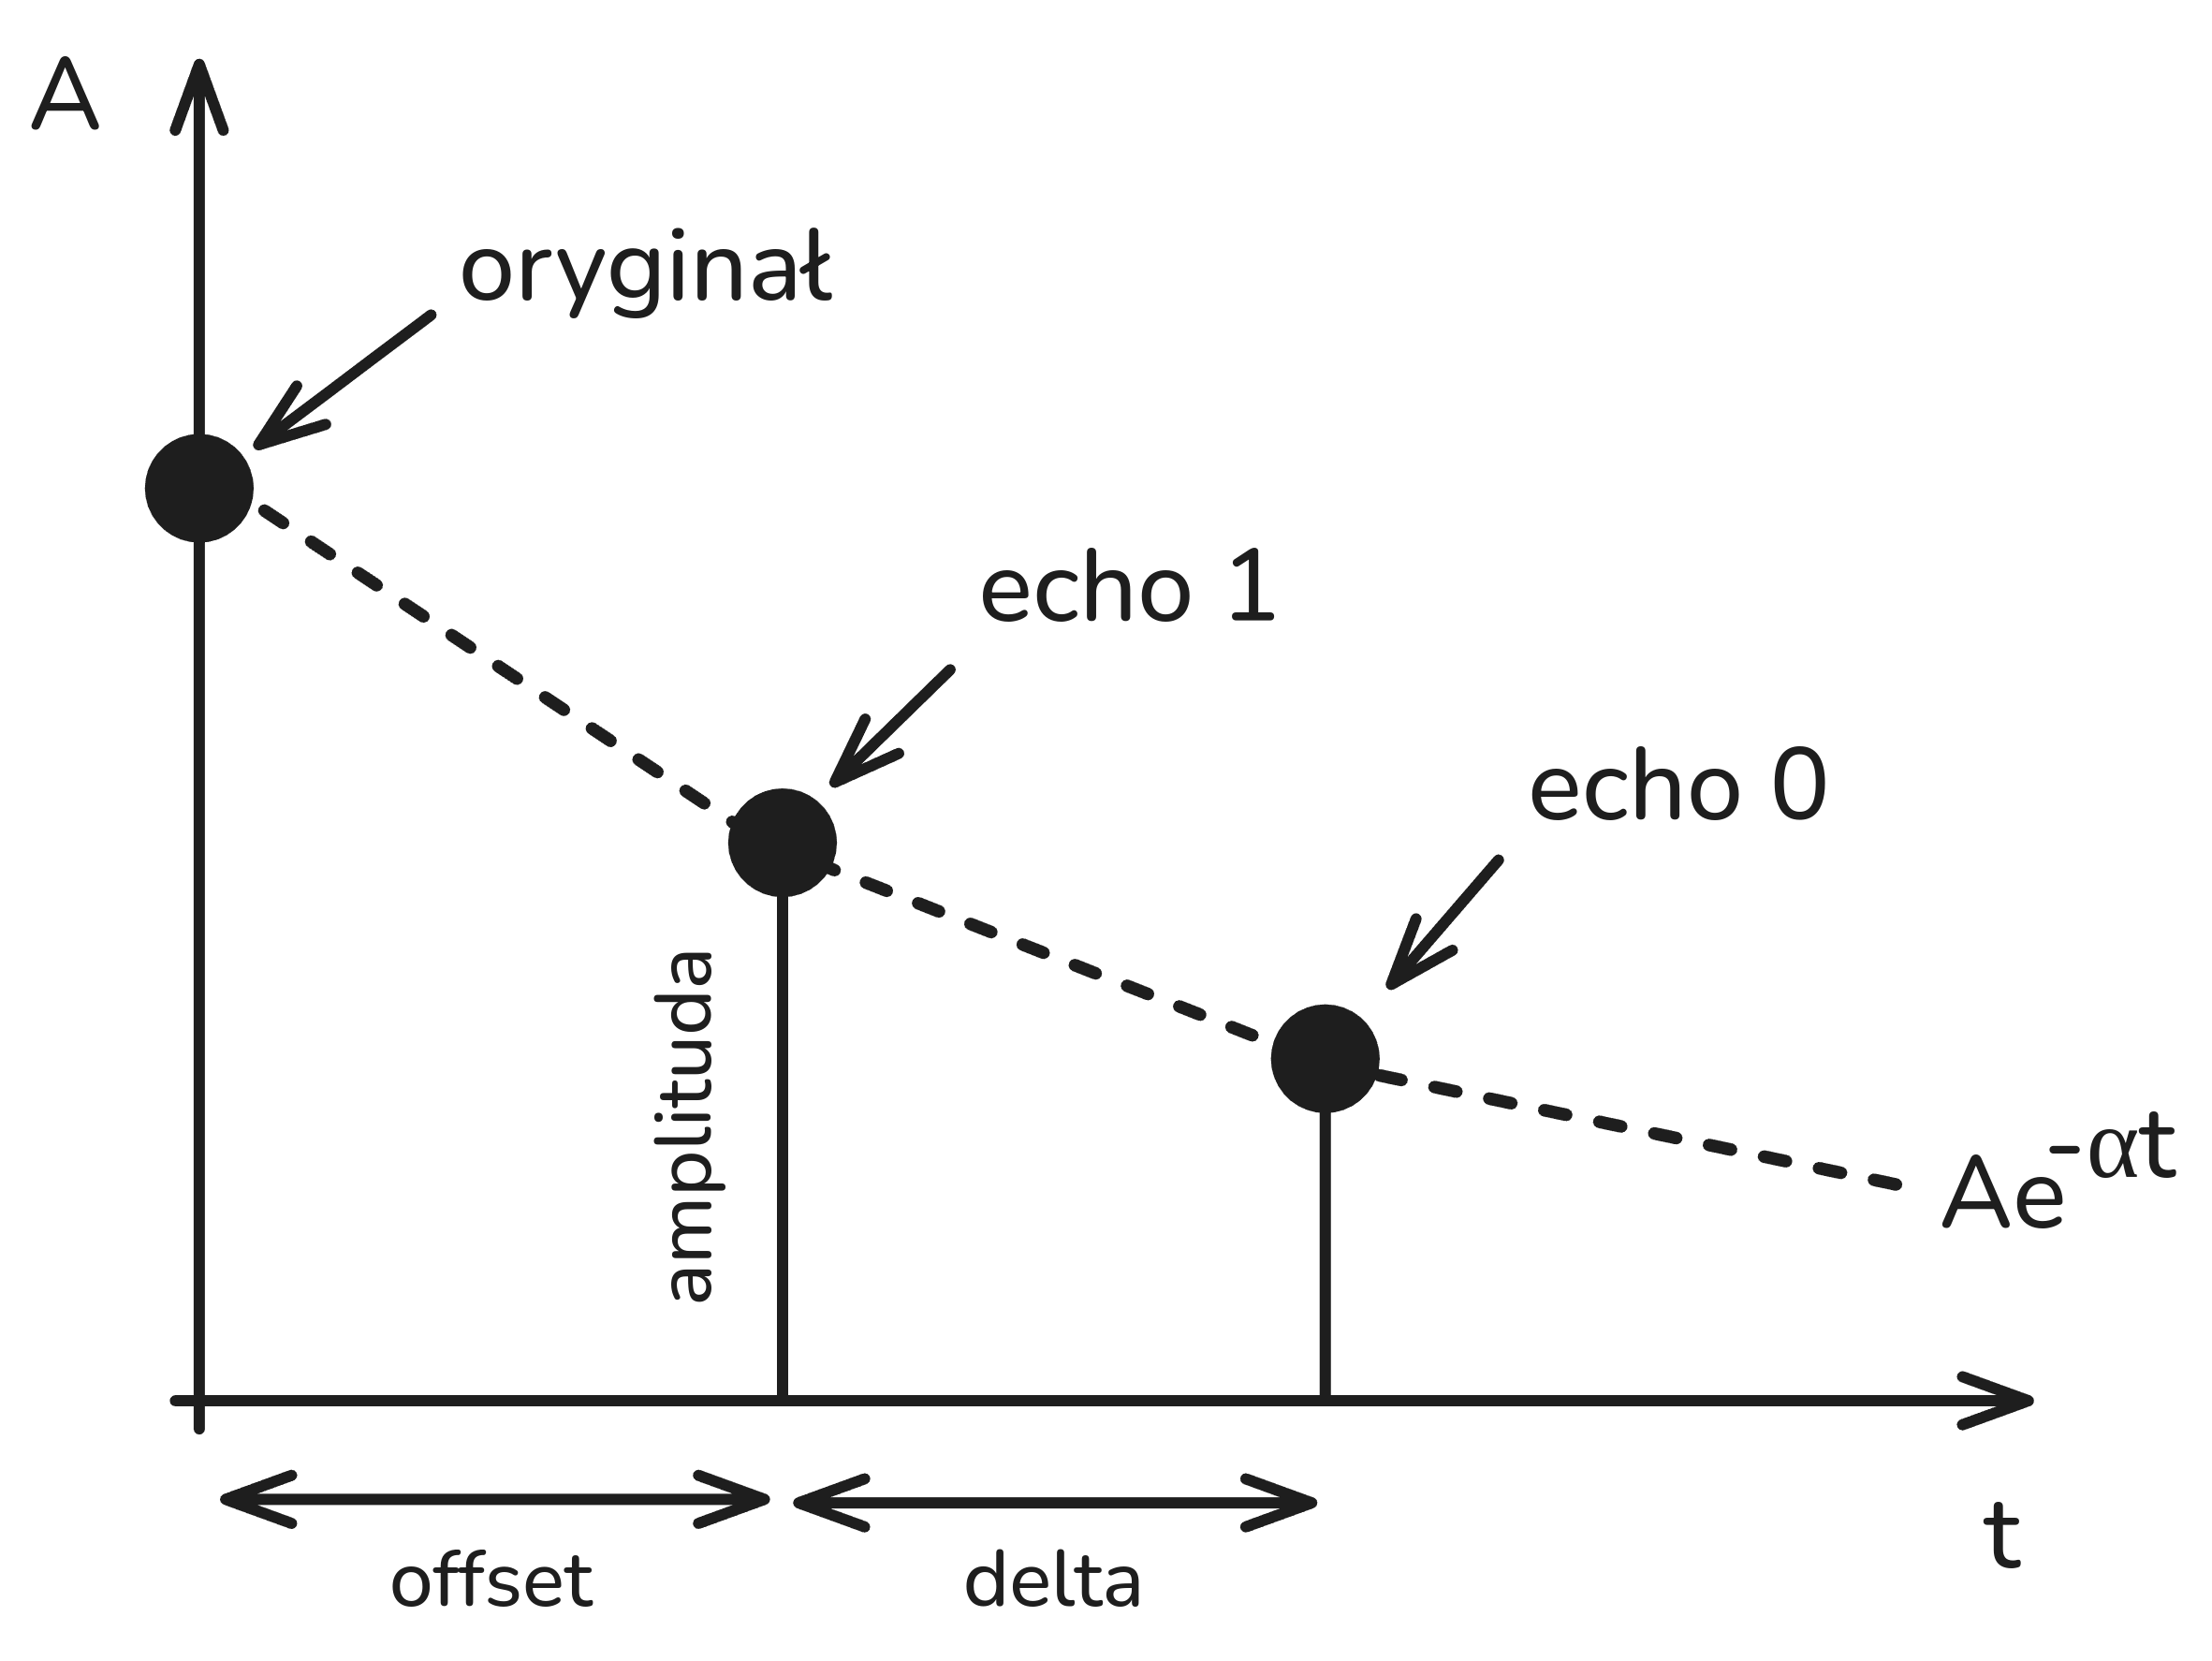
\includegraphics[width=0.6\textwidth]{img/echo-hiding.png}
	\caption{\label{fig:echo-hiding} Parametry EH.}
\end{figure}
\pagebreak


\subsection{Dekodowanie}

Opisany poniżej proces dekodowania został wykonany na przykładzie ukrytego echo o parametrach: $d_1=48$ próbek, $d_0=96$ próbek, i długości segmentu $N=1078$ próbek, w pliku audio z nagraną ludzką mową.

\subsubsection{Analiza cepstralna i cepstrum mocy}

Najczęstszą procedurą wykorzystywaną do wykrywania echa jest analiza cepstralna.
Obliczenie tzw. cepstrum $C_y(n)$ pozwala zidentyfikować opóźnienia dodanego echa, ponieważ zawiera wyraźne szczyty w odpowiadających im pozycjach.

Cepstrum $C_y(n)$ definiowane jest jako odwrotna transformata Fouriera logarytmu widma amplitudowego sygnału:
\begin{equation}
	C_y(n) = \mathcal{F}^{-1} \big(\ln |\mathcal{F}(y(n))|\big),
\end{equation}
gdzie $\mathcal{F}$ oznacza transformatę Fouriera, $y(n)$ to sygnał z ukrytym echem, a $\mathcal{F}^{-1}$ oznacza odwrotną transformatę Fouriera.

Można również zdefiniować tzw. cepstrum mocy (ang. \textit{power cepstrum}), które daje lepsze wyniki niż samo cepstrum \cite{auto_power_cepstrum}. Oblicza się je jako odwrotną transformatę Fouriera logarytmu mocy widma sygnału:
\begin{equation}
	P_{\text{y}}(n) = \left| \mathcal{F}^{-1} \big( \ln |\mathcal{F}(y(n))|^2 \big) \right|^2,
\end{equation}

\begin{lstlisting}[language=Python, caption={Fragment kodu liczącego cepstrum mocy.}]
def power_cepstrum(audio):
    spectrum = np.abs(np.fft.fft(audio)) ** 2
    log_spectrum = np.log(spectrum + np.finfo(float).eps)
    power_cepstrum = np.abs(np.fft.ifft(log_spectrum)) ** 2
    return power_cepstrum
\end{lstlisting}

\begin{figure}[ht!]
	\centering
	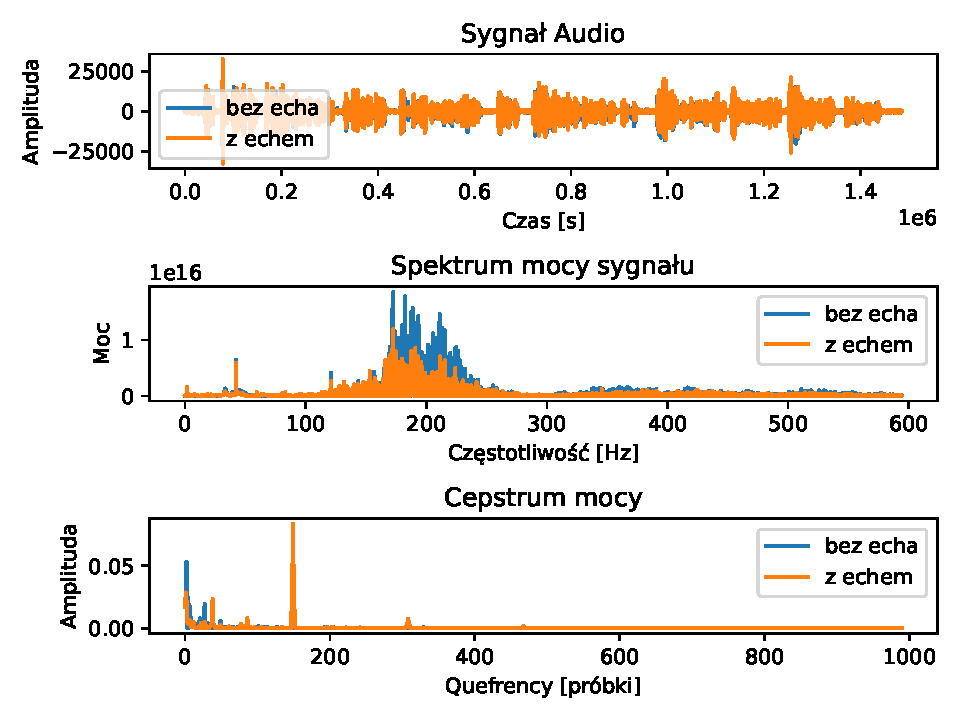
\includegraphics[width=0.9\textwidth]{./img/plot_echo_signal_spectrum_cepstrum.pdf}
	\caption{Porównanie reprezentacji sygnału z echem i bez echa.}
\end{figure}

\subsubsection{Estymacja opóźnień echa}

Dokonując steganalizy jako potencjalny atakujący, nie mamy pojęcia o użytych parametrach do kodowania echem. Natomiast, możliwa jest ich estymacja poprzez wykorzystanie analizy cepstrum mocy z przesuwanym oknem (ang. \textit{sliding window}) \cite{echo_swc}.

W tej metodzie sygnał analizowany jest segment po segmencie za pomocą okna o określonym rozmiarze $\tau$, które przesuwa się po sygnale z krokiem $k$ (\ref{fig:sliding}). Dla każdego segmentu obliczane jest cepstrum mocy, a następnie lokalizowane są szczyty odpowiadające potencjalnym opóźnieniom $d_0$ i $d_1$. Po przesunięciu okna przez cały sygnał tworzy się histogram lokalizacji pików w celu identyfikacji najbardziej prawdopodobnych wartości opóźnień.

\begin{figure}[ht!]
	\centering
	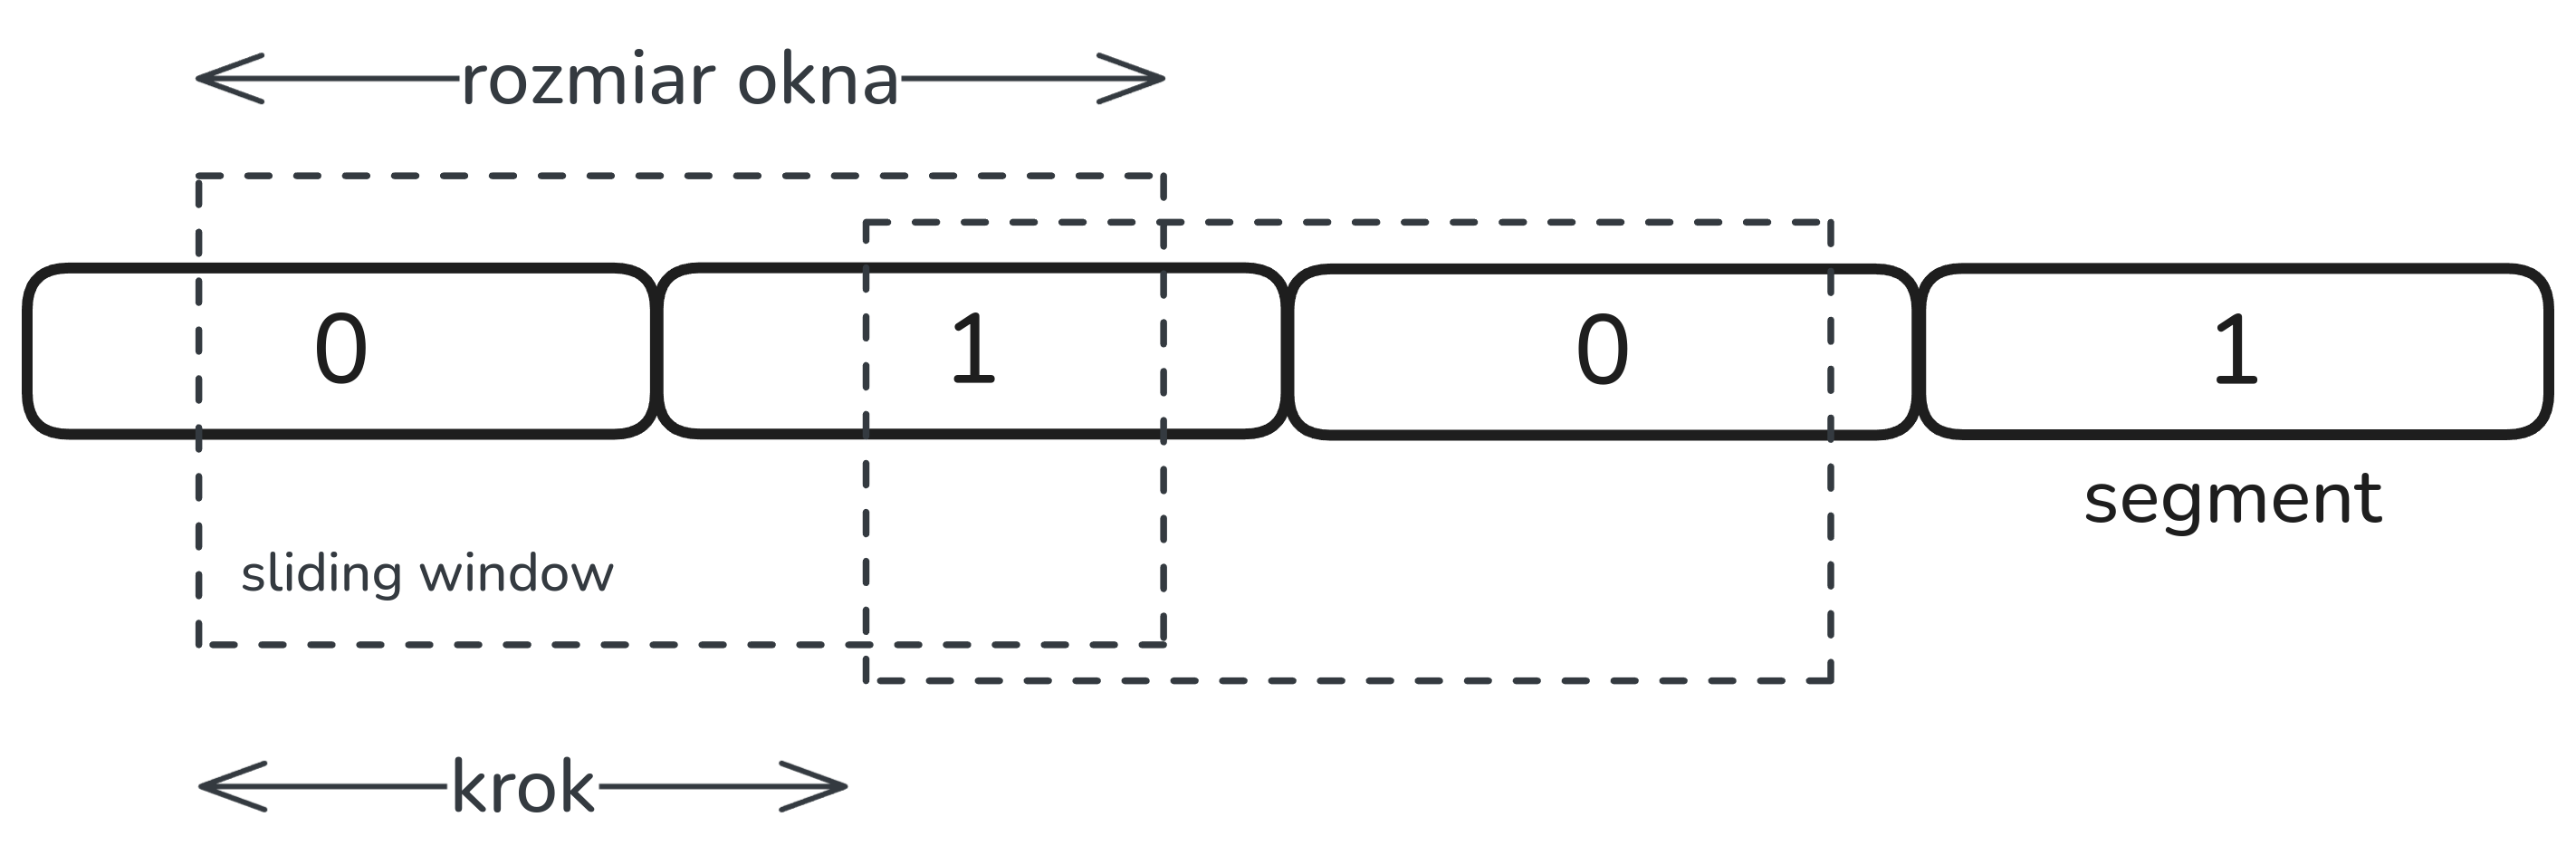
\includegraphics[width=\textwidth]{./img/echo-sliding-window.png}
	\caption{\label{fig:sliding} Wizualizacja algorytmu okna przesuwnego.}
\end{figure}
\pagebreak

Algorytm został zaimplementowany w klasie \verb|EchoDetector|, której wejściowe parametry to:
\begin{itemize}
	\item \verb|window_size| -- długość okna analizy w próbkach,
	\item \verb|step_size| -- krok przesuwania okna w próbkach,
	\item \verb|min_delay| -- minimalny czas opóźnienia, który będzie analizowany,
	\item \verb|max_delay| -- maksymalny czas opóźnienia, który będzie analizowany.
\end{itemize}

Cepstrum mocy jest obliczane dla kolejnych segmentów sygnału, wyznaczanych za pomocą okna przesuwnego, z dodatkowo aplikowaną funkcją Hamminga. Metoda \verb|iter_cepstrums| generuje cepstrum dla kolejnych okien:

\begin{lstlisting}[language=Python, caption={Generator liczący cepstrum mocy dla poszczególnych okien przesuwnych.}]
def iter_cepstrums(self, audio, *, window_size=None, step_size=None):
    window_size = window_size or self.window_size
    step_size = step_size or self.step_size
    for idx in range(0, (audio.size - window_size) + 1, step_size):
        window = audio[idx : idx + window_size]
        window = window * np.hamming(window_size)
        yield power_cepstrum(window)
\end{lstlisting}

Na podstawie obliczonego cepstrum, metoda \verb|estimate_delays| wyznacza histogram lokalizacji maksimów w przedziale \verb|min_delay|--\verb|max_delay|. Dwa najczęściej występujące maksima (\verb|d0| i \verb|d1|) są uznawane za potencjalne opóźnienia echa:

\begin{lstlisting}[language=Python, caption={Tworzenie histogramu z lokalizacji pików.}]
counts, bins = np.histogram(
    peak_locations,
    bins=(self.max_delay - self.min_delay),
    range=(self.min_delay, self.max_delay),
)
top_2 = np.argsort(counts)[-2:]
d0, d1 = bins[top_2]
\end{lstlisting}

\subsubsection{Współczynnik CPLAR}

Jedną z kluczowych wielkości oceniających jakość detekcji opóźnień jest współczynnik \textbf{CPLAR} (\textit{Cepstrum Peak Location Aggregation Rate}) \cite{echo_swc}. Jest definiowany jako stosunek liczby okien cepstrum, w których piki zostały poprawnie zlokalizowane w pozycjach $d_0$ lub $d_1$, do całkowitej liczby analizowanych okien.

\begin{lstlisting}[language=Python, caption={Obliczanie współczynnika CPLAR.}]
cplar = sum(counts[top_2]) / len(peak_locations)
\end{lstlisting}

\subsubsection{Estymacja długości segmentu}

Po otrzymaniu opóźnień echa można wyznaczyć długość segmentu w przybliżony sposób, poprzez iterowanie po potencjalnych długościach i wyznaczanie na podstawie każdego segmentu średnią sumę wartości cepstrum w lokalizacjach \verb|d0| i \verb|d1| \cite{echo_swc}:

\begin{lstlisting}[language=Python, caption={Średnia z sum wartości pików z każdego segmentu.}]
avg_sum = np.mean(
    [
        cepstrum[d0] + cepstrum[d1]
        for cepstrum in self.iter_cepstrums(
            audio,
            window_size=est_length,
            step_size=est_length,
        )
    ]
)
\end{lstlisting}

Ostateczna, estymowana długość segmentu to ta, dla której średnia suma wartości mocy w lokalizacjach \verb|d0| i \verb|d1| jest największa (\ref{fig:segment-len}):

\begin{lstlisting}[language=Python, caption={Branie długości, której odpowiada średnia suma o maksymalnej wartości}]
return lengths[np.argmax(avg_sums)]
\end{lstlisting}

\begin{figure}[ht!]
	\centering
	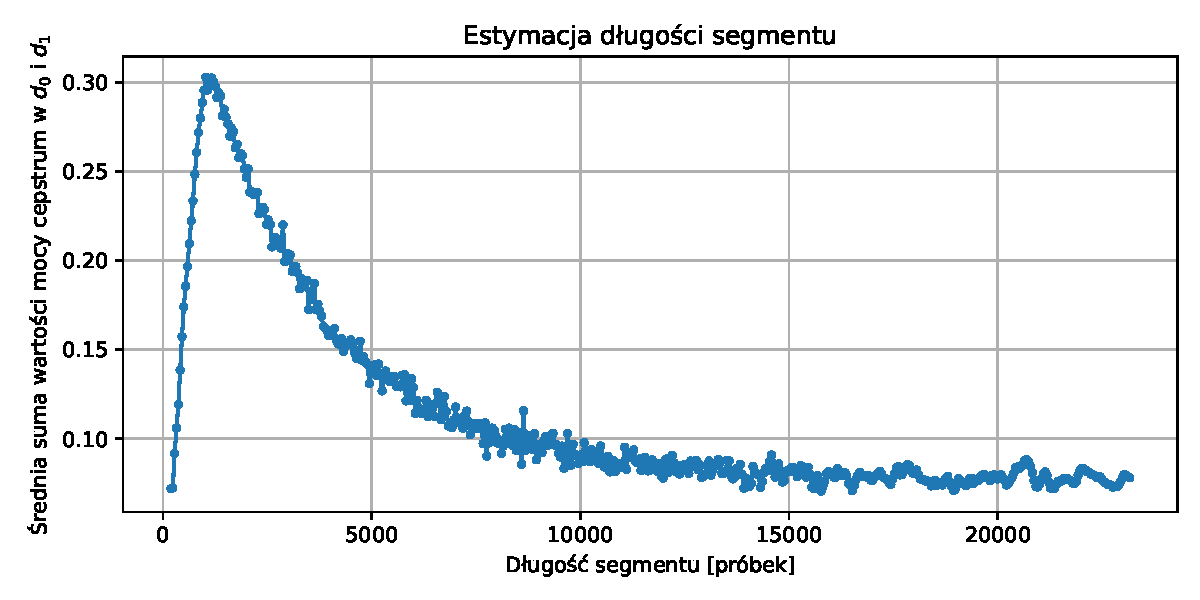
\includegraphics[width=\textwidth]{./img/plot_echo_segment_length.pdf}
	\caption{\label{fig:segment-len} Wykres średniej sumy pików od badanej, potencjalnej długości segmentu.}
\end{figure}
\pagebreak

Na koniec, znając już wszystkie potrzebne parametry można obliczyć długości segmentów $N$, z jakimi zakodowana jest wiadomość.

\begin{lstlisting}[language=Python, caption={Ostateczna procedura dekodowania wiadomości.}]
num_bits = result.size // segment_len
bits = np.zeros(num_bits).astype(np.uint8)

for idx, cepstrum in zip(
    range(num_bits),
    detector.iter_cepstrums(
        result,
        window_size=segment_len,
        step_size=segment_len,
    ),
):
    peak_one = d1 < cepstrum.size and cepstrum[d1] or 0
    peak_zero = d0 < cepstrum.size and cepstrum[d0] or 0
    bits[idx] = int(peak_one < peak_zero)
\end{lstlisting}

\subsection{Podsumowanie}

W ramach projektu zaimplementowano algorytmy pozwalające na detekcję opóźnień $d_0$ i $d_1$, oraz oszacowanie długości segmentów $N$. Kluczowe równania, takie jak obliczanie cepstrum mocy oraz proces analizy z przesuwanym oknem, zostały zaimplementowane w środowisku Python.
